\begin{comment}
------------------------------------------------------------------------------------------
\end{comment}
\chapter{RO-SLAM}\label{ch:ro_slam}

Nachdem im vorherigen Kapitel die \Glspl{uwbm} für die Entfernungsmessung erstellt worden sind, wird jetzt nur noch eine Roboterplattform benötigt die mit einem Tag ausgestattet werden kann. Welche Hardwareplattform eingesetzt wird und von welchen Softwaremodulen diese gesteuert wird, folgt in den nächsten Abschnitten.

\begin{comment}
--------------------------------------------------------------------------------
- Einsatz mobiler Roboter in der Logistik am Beispiel des Robotino
	- http://www.r-moehrle.de/wissenschaftlicheArbeiten/robotino1.pdf
\end{comment}
\section{Roboterplattform}

Um die Messungen für den \Gls{roslam} aufzuzeichnen wird eine Roboterplattform benötigt auf der das \Gls{uwbm} montiert werden kann. Zusätzlich wird noch eine Reihe weiterer Sensoren benötigt, die im Folgenden vorgestellt werden.

Also Roboterplattform dient dabei der Robotino 2 von \textit{Festo Didactic}. Er gehört zur Klasse der holonomen Roboter, d.h. seinen Bewegungsmöglichkeiten unterliegen keinerlei Einschränkungen im zweidimensionalen Raum. Ermöglicht wird das, durch drei voneinander unabhängig arbeitenden omnidirektionalen Antriebseinheiten. Jede der drei Antriebseinheiten verfügt über einen Inkrementalgeber, mit dem sich abschätzen lässt, wie weit der Robotino gefahren ist. Um den Fehler der Inkrementalgeber in Kurvenfahrten zu reduzieren wird das digitale Gyroskop\footnote{Model: CruizCore XG1000 / XG1010} von \textit{Microinfinity} eingesetzt. Gesteuert wird der Robotino über eine \SI{300}{\MHz} starke Verarbeitungseinheit auf Basis eines Linux Betriebssystems mit einem Echtzeitkernel. \cite{festo2007robotinomanual}

An der höchsten Position des Robotinos befindet sich ein 2D-LiDAR-Sensor\footnote{Model: TiM571-2050101} der Firma \textit{Sick}. Mit einem Öffnungswinkel von \SI{270}{\degree} und einem Arbeitsbereich von \SIrange{0.05}{25}{\meter} ist es möglich, genaue Belegungskarten der Umgebung zu erstellen. \cite{sick2016operatingmanual}

Die Verarbeitungseinheit des Robotinos ist leistungsfähig genug um die anstehenden Steuerungsaufgaben zu erfüllen. Jedoch ist diese von leistungshungrigen Anwendungen wie dem \Gls{roslam} überfordert. Aus diesem Grund wird eine zusätzliche Verarbeitungseinheit\footnote{Model: NUC5i7RYH} mit einem Intel Core i7\footnote{5. Generation des Intel Core i7-5557U Prozessor mit bis zu \SI{3.4}{\GHz}. \cite{intel2015nucproductbrief}} verwendet.

Die Fahrbefehle werden dem Robotino über einen Xbox Wireless Controller übermittelt.

\begin{figure}[h]
	\centering
	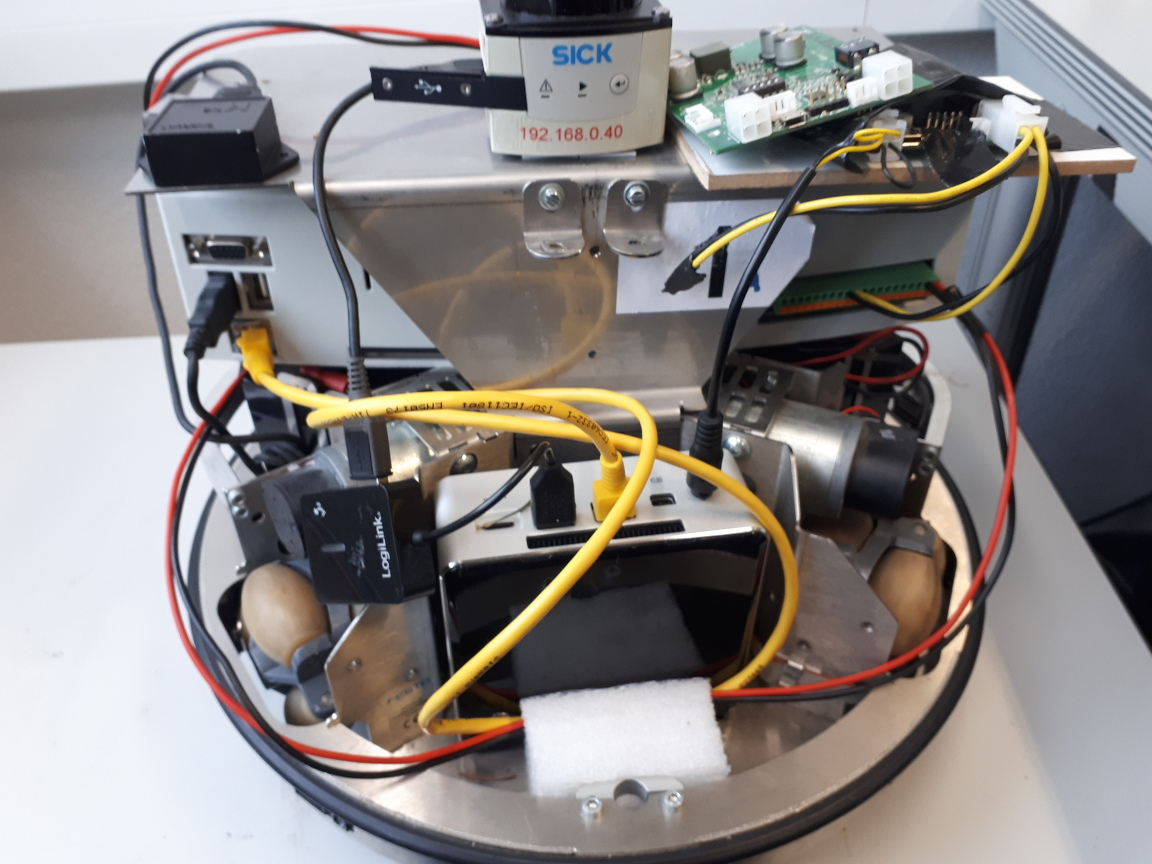
\includegraphics[width=0.5\textwidth]{robotino_front}
	\caption{[todo] Frontansicht des fertig aufgebauten Robotinos.}
	\label{fig:robotino_front}
\end{figure}


\begin{comment}
--------------------------------------------------------------------------------
- Kurzbeschreibung der Modulfunktion
- Welche Funktion erfüllt dieses Modul
- Welche ROS-Messages/-Topics/-Services bietet dieses Modul
\end{comment}
\section{Softwarearchitektur [todo]}


\begin{comment}
--------------------------------------------------------------------------------
- Begrifflichkeiten wie Topic, Sessage, Service usw. wurden bereits im Grundlagenkapitel geklärt.
- TODO: Grundlagen ROS: URDF, Lauch-Files, TF-Tree (odom, base_link, map?)
\end{comment}
\subsection{ROS Hauptmodule [todo]}


\begin{comment}
--------------------------------------------------------------------------------
"max_linear_vel", "min_linear_vel", "max_angular_vel", "min_angular_vel"

<node name="robotino_node" pkg="robotino_node" type="robotino_node" output="screen">
	<param name="hostname" value="$(arg hostname)" />
	<param name="max_linear_vel" value="0.5" />
	<param name="min_linear_vel" value="0.05" />
	<param name="max_angular_vel" value="3.0" />
	<param name="min_angular_vel" value="0.1" />
	<remap from="robotino_joint_states" to="joint_states" />
</node>

OmniDriveROS::OmniDriveROS()
{
	cmd_vel_sub_ = nh_.subscribe("cmd_vel", 1, &OmniDriveROS::cmdVelCallback, this);
}
\end{comment}
\subsubsection{Robotino robotino\_node}

Kommunikation mit der Robotino-Steuereinheit, Auslesen der Sensoren, Bewegungssteuerung über das Topic cmd\_vel, begrenzen der maximalen Parameter.


\begin{comment}
--------------------------------------------------------------------------------

odometry_pub_ = nh_.advertise<nav_msgs::Odometry>("odom", 1, true);

Transformation: odom <- base_link
odometry_transform_broadcaster_.sendTransform( odometry_transform_ );

reset_odometry_server_ = nh_.advertiseService("reset_odometry",
			&OdometryROS::resetOdometryCallback, this);
			
<node name="robotino_odometry_node" pkg="robotino_node" type="robotino_odometry_node" output="screen">
	<param name="hostname" value="$(arg hostname)" />
</node>
\end{comment}
\subsubsection{robotino\_odometry\_node}

Erzeugt die Transformation zwischen odom und base\_link Koordinatensystem.
Sorgt dafür, dass die Odometry--Nachrichten vom Robotino ins ROS--System veröffentlicht werden.



\begin{comment}
--------------------------------------------------------------------------------
<param name="robot_description" textfile="$(find robotino_description)/urdf/robotino.urdf" />
<node pkg="robot_state_publisher" type="state_publisher" name="robot_state_publisher" output="screen">
	<param name="publish_frequency" type="double" value="20.0" />
</node>

- Bild von dem Robotino + TF Tree
\end{comment}
\subsubsection{state\_publisher}




\begin{comment}
--------------------------------------------------------------------------------
- http://wiki.ros.org/teleop_twist_joy
- http://yardbot.ca/2014/10/writing-custom-joystick-teleop-node-ros/

<node pkg="joy" type="joy_node" name="joy_node" output="screen">
	<param name="dev" type="string" value="/dev/input/js0" />
</node>

Published Topics
- joy (joy/Joy): Outputs the joystick state.
- joy (sensor_msgs/Joy): Outputs the joystick state.

Parameters
~dev (string, default: /dev/input/js0): Linux joystick device from which to read joystick events.
~autorepeat_rate (double, default: 0.0 (disabled)): Rate in Hz at which a joystick that has a non-changing state will resend the previously sent message.

\end{comment}
\subsubsection{joy\_node}


ROS driver for a generic Linux joystick. The joy package contains joy\_node, a node that interfaces a generic Linux joystick to ROS. This node publishes a "Joy" message, which contains the current state of each one of the joystick's buttons and axes.





\begin{comment}
--------------------------------------------------------------------------------
rospy.Subscriber('joy', Joy, callback)

# TurtleSim commands
# http://wiki.ros.org/ROS/Tutorials/UnderstandingTopics
pub = rospy.Publisher('/cmd_vel', Twist, queue_size=60)
\end{comment}
\subsubsection{xbox\_teleop.py}

Erzeugt aus der joy-Message eine cmd\_vel-Message.





\begin{comment}
--------------------------------------------------------------------------------
A ROS driver for the SICK TiM series of laser scanners.
Auslesen des 2D-LiDAR-Sensors und erstellen einer 
TIM571-2050101 (P/N 1075091); frequency: 15 Hz, angular resolution: 0.333°, range: 25m; see sick_tim571_2050101.launch

scan (sensor_msgs/LaserScan): The published laser scans.

~frame_id (str, default: laser): The TF frame in which laser scans will be returned.
\end{comment}
\subsubsection{sick\_tim}


\url{http://wiki.ros.org/sick_tim}


\begin{comment}
--------------------------------------------------------------------------------
pub = rospy.Publisher('beacon', ObservationRangeBeacon, queue_size=10)
pub_raw = rospy.Publisher('beacon_raw', Beacon, queue_size=10)

antenna_delay = rospy.get_param('~antenna_delay', 16450)
sensor_frame_id = rospy.get_param('~sensor_frame_id', 'uwb_reciever_link')
serial_port = rospy.get_param('~serial_port', '/dev/CP2104_Friend')
\end{comment}
\subsubsection{beacon\_publisher\_node}




\begin{comment}
--------------------------------------------------------------------------------
\end{comment}
\subsection{ROS Hilfsmodule [todo]}

- Erstellen einer Umgebungskarte und der Trajektorie in der Umgebungskarte.
- Vergleichen der Roboter--Odometrie mit zwei Laser--Odometrien.


\begin{comment}
--------------------------------------------------------------------------------
<node pkg="hector_mapping" type="hector_mapping" name="hector_mapping" output="screen">
  <param name="scan_topic" value="scan" />
  <param name="base_frame" value="base_link" />
  <param name="odom_frame" value="odom" />
  <param name="map_frame" value="map" />

  <param name="pub_map_odom_transform" value="true" />

  <param name="map_resolution" value="0.02" />
  <param name="laser_min_dist" value="0.05" />
	<param name="laser_max_dist" value="30.0" />
</node>
- \url{http://wiki.ros.org/hector_mapping}
- hector_mapping is a SLAM approach that can be used without odometry as well as on platforms that exhibit roll/pitch motion (of the sensor, the platform or both). It leverages the high update rate of modern LIDAR systems like the Hokuyo UTM-30LX and provides 2D pose estimates at scan rate of the sensors (40Hz for the UTM-30LX). While the system does not provide explicit loop closing ability, it is sufficiently accurate for many real world scenarios. The system has successfully been used on Unmanned Ground Robots, Unmanned Surface Vehicles, Handheld Mapping Devices and logged data from quadrotor UAVs.
- Bild vom OccupanyGrid
\end{comment}
\subsubsection{hector\_mapping}



\begin{comment}
--------------------------------------------------------------------------------
\end{comment}
\subsubsection{hector\_trajectory\_server}

Mit diesem Modul ist es möglich die gefahrene Trajektorie eine Roboters in einem bestimmten Koordinatensystem auszugeben. Hierfür muss im TF--Tree eine Verbindung zwischen dem \textit{source\_frame\_name}(base\_link) und dem \textit{target\_frame\_name}(odom oder map) bestehen. Die Trajektorie bezieht sich mit ihren Koordinaten auf das target\_frame und ist vom Datentyp nav\_msgs/Path.

Über einen Service lässt die sich Trajektorie auch abfragen: \textit{rosservice call /trajectory}

\url{http://wiki.ros.org/hector_trajectory_server}

\url{http://docs.ros.org/api/nav_msgs/html/msg/Path.html}

\begin{listing}
	\begin{minted}[frame=single]{xml}
<node 
  name="hector_trajectory_server"
  pkg="hector_trajectory_server"
  type="hector_trajectory_server"
  output="screen">

  <param name="target_frame_name" value="map"/>
  <param name="source_frame_name" value="base_link" />
  <param name="trajectory_update_rate" value="10.0" />
  <param name="trajectory_publish_rate" value="10"/>
</node>
	\end{minted}
	\unskip
	\caption{Konfiguration der hector\_trajectory\_server--Nodes.}
	\label{lst:hector_trajectory_server_node}
\end{listing}


\begin{comment}
--------------------------------------------------------------------------------
\end{comment}
\subsubsection{rf2o\_laser\_odometry}

\url{http://wiki.ros.org/rf2o}


\begin{comment}
--------------------------------------------------------------------------------
    <node
        if="$(arg enable_laser_scan_matcher)"
        pkg="laser_scan_matcher" type="laser_scan_matcher_node" name="laser_scan_matcher_node"
        output="screen">

        <param name="base_frame" value="base_link"/>
        <param name="fixed_frame" value="odom" />
        <param name="use_odom" value="true" />
        <param name="use_imu" value="false" />
    </node>
\end{comment}
\subsubsection{laser\_scan\_matcher}

\url{http://wiki.ros.org/laser_scan_matcher}





\begin{comment}
--------------------------------------------------------------------------------
\subsubsection{gmapping}

- This package contains a ROS wrapper for OpenSlam's Gmapping.
- The gmapping package provides laser-based SLAM (Simultaneous Localization and Mapping), as a ROS node called slam\_gmapping.
- Using slam\_gmapping, you can create a 2-D occupancy grid map from laser and pose data collected by a mobile robot.
\url{http://wiki.ros.org/gmapping}

Benötigt eine TF--Transformation zwischen base\_link und odom. Mittels der Odometry und dem Laser--Scans erzeugt er eine TF--Transformation zwischen map und odom.
\end{comment}



\begin{comment}
--------------------------------------------------------------------------------
\subsubsection{Vergleich der Trajektorie von Odom und rf2o}

- Trajektorie der Robotino--Odometry bestimmen.
- Herausfiltern der Odometry Nachrichten aus den Bag--Dateien
- Odometry aus den Laser--Scans bestimmen und Trajektorie aufzeichen.
- Trajektorien vergleichen
\end{comment}



\begin{comment}
--------------------------------------------------------------------------------
- ros
	- <node pkg="mrpt_rbpf_slam" type="mrpt_rbpf_slam" name="mrpt_rbpf_slam" output="screen" />
- mrpt
	- rbpf_slam.ini
- https://www.mrpt.org/list-of-mrpt-apps/application-rbpf-slam/
	- It is actually a front-end to the class mrpt::slam::CMetricMapBuilderRBPF. All the parameters to the algorithm are passed through a configuration file in the command line. The filter processes actions and observations from a rawlog file and optionally generates a number of files describing the evolution of the filter and the maps.
	- The mathematical background of RBPF-based SLAM and to see an updated list of the implemented RBPF-SLAM solutions can be found in this tutorial page.
	- http://mrpt.ual.es/reference/devel/classmrpt_1_1slam_1_1_c_metric_map_builder_r_b_p_f.html
	- MC / SOG
	- https://www.mrpt.org/tutorials/slam-algorithms/rangeonly_slam/
	
	
pub_map_ = n_.advertise<nav_msgs::OccupancyGrid>("map", 1, true);
// robot pose
pub_Particles_ = n_.advertise<geometry_msgs::PoseArray>("particlecloud", 1, true);
 / ro particles poses
pub_Particles_Beacons_ = n_.advertise<geometry_msgs::PoseArray>("particlecloud_beacons", 1, true);
	
if (lstSources[i].find("scan") != std::string::npos)
    {
      sensorSub_[i] = n_.subscribe(lstSources[i], 1, &PFslamWrapper::laserCallback, this);
    }
    else
    {
      sensorSub_[i] = n_.subscribe(lstSources[i], 1, &PFslamWrapper::callbackBeacon, this);
    }
    
    
void PFslamWrapper::odometryForCallback(CObservationOdometry::Ptr& _odometry, const std_msgs::Header& _msg_header)
{
  mrpt::poses::CPose3D poseOdom;
  if (this->waitForTransform(poseOdom, odom_frame_id, base_frame_id, _msg_header.stamp, ros::Duration(1)))
	
\end{comment}
\subsection{MRPT Modul [todo]}








